\documentclass[11pt]{article}
\usepackage[margin=1in]{geometry}
\usepackage{amsmath,amssymb}
\usepackage{graphicx}
\usepackage{enumitem}
\usepackage{comment}
\usepackage{bookmark}
\hypersetup{
  pdftitle={PSET 2: Limits and Derivatives},
  hidelinks}

\title{PSET 2: Limits and Derivatives}
\author{}
\date{\vspace{-2.5em}}

\newcounter{problem}
\newcommand{\problem}[1]{\stepcounter{problem}\section*{Problem \theproblem: #1}}

\begin{document}
\maketitle

% Shared assignment questions (header block).
% Include at the top of any problem set with:  % Shared assignment questions (header block).
% Include at the top of any problem set with:  % Shared assignment questions (header block).
% Include at the top of any problem set with:  \input{assignment-qs}
\section*{Assignment Qs}

\begin{itemize}
\item Name
\item How long did this problem set take you (round to nearest hour)? \quad
  0-1 hour \ 2-3 hours \ 4-5 hours \ 5+ hours
\item How difficult was this problem set? \quad
  very easy \ 1 \ 2 \ 3 \ 4 \ 5 \ very challenging
\end{itemize}

\section*{Assignment Qs}

\begin{itemize}
\item Name
\item How long did this problem set take you (round to nearest hour)? \quad
  0-1 hour \ 2-3 hours \ 4-5 hours \ 5+ hours
\item How difficult was this problem set? \quad
  very easy \ 1 \ 2 \ 3 \ 4 \ 5 \ very challenging
\end{itemize}

\section*{Assignment Qs}

\begin{itemize}
\item Name
\item How long did this problem set take you (round to nearest hour)? \quad
  0-1 hour \ 2-3 hours \ 4-5 hours \ 5+ hours
\item How difficult was this problem set? \quad
  very easy \ 1 \ 2 \ 3 \ 4 \ 5 \ very challenging
\end{itemize}


\problem{Limits: left, right, and at a point}

Given that\footnote{Grimmer 2012 HW 2.4}
\[
\lim_{x \to a} f(x) = -3, \quad
\lim_{x \to a} g(x) = 0, \quad
\lim_{x \to a} h(x) = 8
\]
find the limits that exist. If a limit does not exist, explain why.

\begin{enumerate}[label=\alph*.]
\item \(\lim_{x \to a} \left[ f(x) + h(x) \right]\)



\item \(\lim_{x \to a} \dfrac{g(x)}{f(x)}\)


\item \(\lim_{x \to a} \dfrac{f(x)}{g(x)}\)


\item \(\lim_{x \to a} \dfrac{2 f(x)}{h(x) - f(x)}\)

\end{enumerate}

\problem{Find even more limits}

Find the following limits:\footnote{Grimmer 2012 HW 2.4(b)}

\begin{enumerate}[label=\alph*.]
\item \(\lim_{x \to -4} \dfrac{x^2 + 5x + 4}{x^2 + 3x - 4}\)


\item \(\lim_{x \to 4^-} \sqrt{16 - x^2}\)

\end{enumerate}

\problem{Check for discontinuities}

Which of the following functions are continuous? If a function is not
continuous, where are the discontinuities?\footnote{Gill 1.9}

\begin{enumerate}[label=\alph*.]
\item \(f(x) = \dfrac{9x^3 - x}{(x - 1)(x + 1)}\)


\item \(f(x) = e^{-x^2}\)


\item \(f(x) = \begin{cases}
  x^3 + 1, & x > 0 \\
  -x^2, & x \leq 0
\end{cases}\)

\end{enumerate}

\problem{Find finite limits}

Find the following finite limits:\footnote{Gill 5.1}

\begin{enumerate}[label=\alph*.]
\item \(\lim_{x \to 1} \left[ \dfrac{x^4 - 1}{x - 1} \right]\)
\end{enumerate}

\problem{Find infinite limits}

Find the following infinite limits:\footnote{Gill 5.3 and 5.8}

\begin{quote}
Hint: use \textbf{L'H\^{o}pital's rule} to switch from
\(\lim_{x \to \infty} \left( \dfrac{f(x)}{g(x)} \right)\) to
\(\lim_{x \to \infty} \left( \dfrac{f'(x)}{g'(x)} \right)\).
\end{quote}

\begin{enumerate}[label=\alph*.]

\item \(\lim_{x \to \infty} \left[ \dfrac{2^x - 3}{2^x + 1} \right]\)


\item \(\lim_{x \to \infty} \left[ \dfrac{3^x}{x^3} \right]\)
\end{enumerate}

\problem{Assess continuity and differentiability}

For each of the following functions, state whether it is continuous
and/or differentiable at the point where its two formulas
meet.\footnote{Simon and Blume 2.16}

\begin{enumerate}[label=\alph*.]
\item \(f(x) = \begin{cases}
  x^2, & x \geq 0 \\
  -x^2, & x < 0
\end{cases}\)


\item \(f(x) = \begin{cases}
  x^3, & x \leq 1 \\
  x, & x > 1
\end{cases}\)

\end{enumerate}

\problem{Calculate derivatives}

Recall the differentiation rules:
\[
\begin{aligned}
\left[ k f(x) \right]' &= k f'(x)
  && \mbox{constant multiple} \\
\left[ f(x) \pm g(x) \right]' &= f'(x) \pm g'(x)
  && \mbox{sum} \\
\left[ f(x) g(x) \right]' &= f'(x) g(x) + f(x) g'(x)
  && \mbox{product} \\
\left[ \dfrac{f(x)}{g(x)} \right]'
  &= \dfrac{f'(x) g(x) - f(x) g'(x)}{\left[ g(x) \right]^2}, \quad g(x) \neq 0
  && \mbox{quotient} \\
\left[ x^k \right]' &= k x^{k-1}
  && \mbox{power}
\end{aligned}
\]

Differentiate the following functions:\footnote{Grimmer HW2.3}

\begin{enumerate}[label=\alph*.]
\item \(f(x) = 4x^3 + 2x^2 + 5x + 11\)
\item \(y = \sqrt{30}\)
\item \(h(t) = \log(9t + 1)\)
\item \(f(x) = \log\left(x^2 e^x\right)\)
\item \(h(y) = \left( \dfrac{1}{y^2} - \dfrac{3}{y^4} \right)\left(y + 5y^3\right)\)
\item \(g(t) = \dfrac{3t - 1}{2t + 1}\)
\end{enumerate}

\problem{Use the product and quotient rules}

Differentiate the following function twice---once using the product
rule, and once using the quotient rule:\footnote{Grimmer HW2.4}
\[
f(x) = \frac{x^2 - 2x}{x^4 + 6}
\]

\problem{Logarithms and exponential functions}

Compute the derivative of each of the following
functions:\footnote{Simon and Blume 5.8}

\begin{enumerate}[label=\alph*.]
\item \(f(x) = \dfrac{x}{e^x}\)
\item \(h(x) = \dfrac{x}{\log(x)}\)
\end{enumerate}

\problem{Composite functions}

For each of the following pairs of functions \(g(x)\) and \(h(z)\),
write out the composite functions \(g(h[z])\) and \(h(g[x])\). In each
case, describe the domain of the composite
function.\footnote{Simon and Blume 4.1}

\begin{enumerate}[label=\alph*.]
\item \(g(x) = x^2 + 4, \quad h(z) = 5z - 1\)
\item \(g(x) = x^3, \quad h(z) = (z - 1)(z + 1)\)
\end{enumerate}

\problem{Chain rule}

Use the chain rule to compute the derivative of the composite
functions in the previous problem from the derivatives of the two
component functions. Then compute each derivative directly, using your
expression for the composite function. Simplify and compare your
answers.\footnote{Simon and Blume 4.3}

\begin{enumerate}[label=\alph*.]
\item \(g(x) = x^2 + 4, \quad h(z) = 5z - 1\)
\item \(g(x) = x^3, \quad h(z) = (z - 1)(z + 1)\)
\end{enumerate}

\problem{Identify a possible derivative}

A friend shows you the graph of a function \(f(x)\) below.\footnote{Grimmer HW3.6}
Which of the following could be a graph of \(f'(x)\)? For each graph,
explain why it might or might not be the derivative of \(f(x)\).

 \begin{center}
 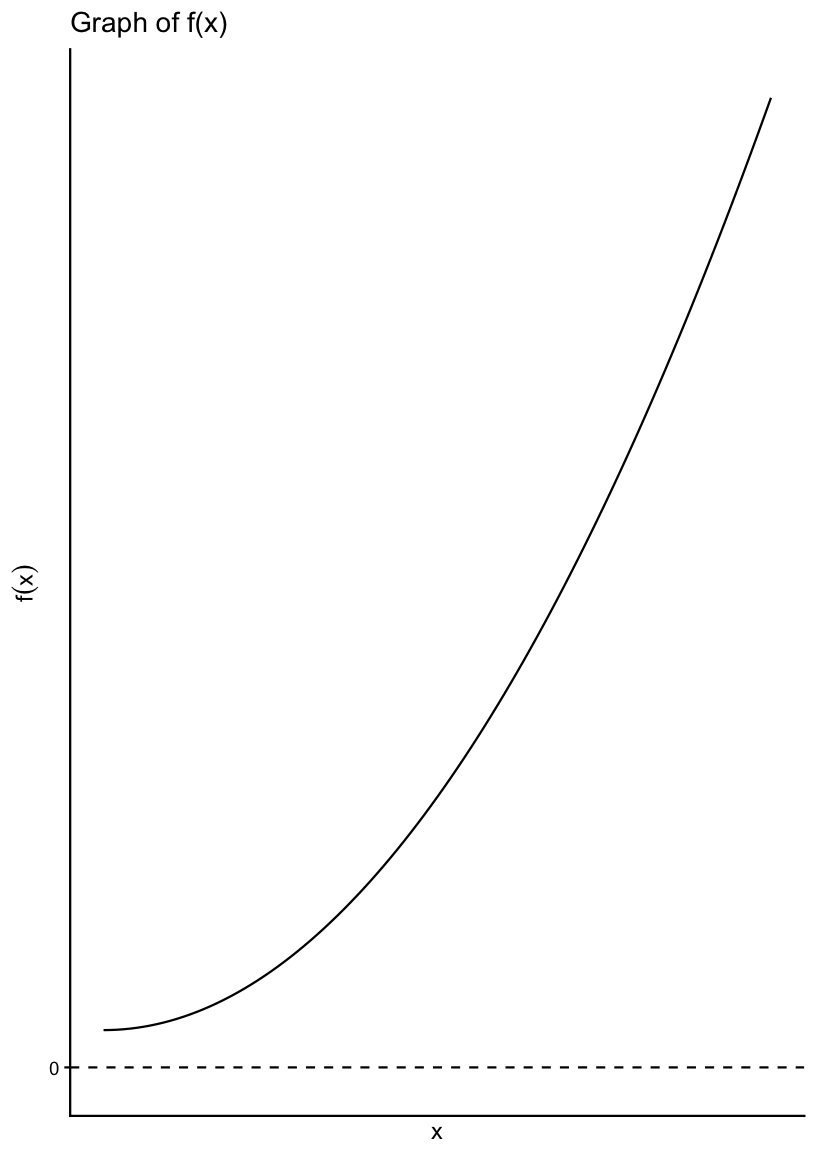
\includegraphics[width=0.55\textwidth]{polynomial.png}
 \end{center}

 \begin{center}
 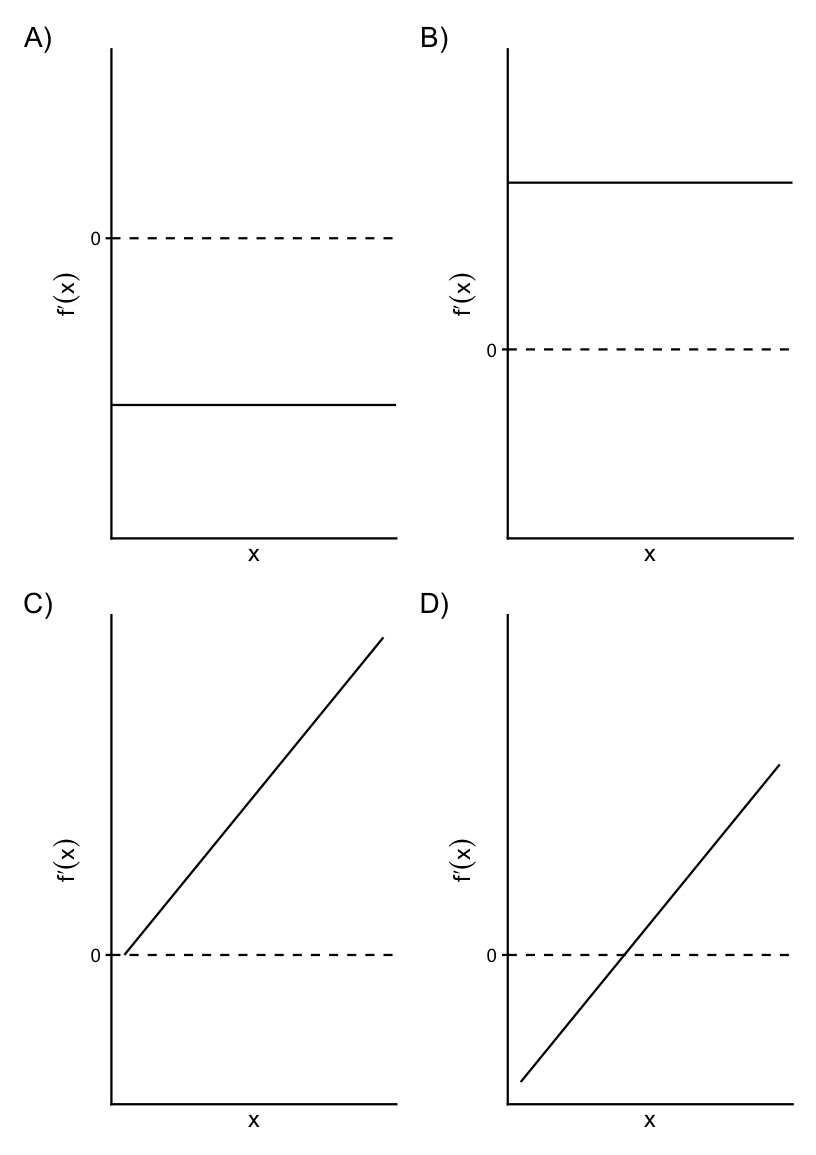
\includegraphics[width=0.9\textwidth]{derivatives.png}
 \end{center}


 % 
 % 
 % library(tidyverse)
 % library(patchwork)
 % 
 % p <- ggplot(data = tibble(x = 0), mapping = aes(x = x)) +
 %   geom_hline(yintercept = 0, linetype = 2) +
 %   xlim(0, 5) +
 %   labs(x = "x", y = expression(f(x))) +
 %   theme_classic() +
 %   theme(axis.text.x = element_blank(),
 %         axis.ticks.x = element_blank())
 % 
 % # Graph of f(x)
 % p +
 %   stat_function(fun = function(x) x^2 + 1) +
 %   scale_y_continuous(breaks = 0, labels = "0") +
 %   ggtitle("Graph of f(x)")
 % 
 % # Candidate derivatives A-D
 % pa <- p +
 %   geom_hline(yintercept = -3) +
 %   labs(y = expression({f * minute}(x)), tag = "A)") +
 %   scale_y_continuous(limits = c(-5, 3), breaks = 0, labels = "0")
 % pb <- p +
 %   geom_hline(yintercept = 3) +
 %   labs(y = expression({f * minute}(x)), tag = "B)") +
 %   scale_y_continuous(limits = c(-3, 5), breaks = 0, labels = "0")
 % pc <- p +
 %   stat_function(fun = function(x) x) +
 %   labs(y = expression({f * minute}(x)), tag = "C)") +
 %   scale_y_continuous(limits = c(-2, 5), breaks = 0, labels = "0")
 % pd <- p +
 %   stat_function(fun = function(x) x - 2) +
 %   labs(y = expression({f * minute}(x)), tag = "D)") +
 %   scale_y_continuous(limits = c(-2, 5), breaks = 0, labels = "0")
 % 
 % pa + pb + pc + pd + plot_layout(ncol = 2)
 % 


% Shared AI and Resources statement.
% Include in any problem set with:  % Shared AI and Resources statement.
% Include in any problem set with:  % Shared AI and Resources statement.
% Include in any problem set with:  \input{ai-statement}
\section*{AI and Resources statement}

Please list (in detail) all resources you used for this assignment. If
you worked with people, list them here as well. It is not enough to say
that you used a resource for help, you need to be specific on the link
and \emph{how} it was helpful. W/R/T gen AI tools (including GPT,
Claude, etc.) you cannot use them to do work on your behalf---you
cannot put in any of the questions, etc. You can ask for help on logic
/ sample problems. If you do use GPT or other AI tools, you need to
provide a link to your chat transcript. Any suspected academic
integrity violations will be immediately reported to the Dean of
Students.

\section*{AI and Resources statement}

Please list (in detail) all resources you used for this assignment. If
you worked with people, list them here as well. It is not enough to say
that you used a resource for help, you need to be specific on the link
and \emph{how} it was helpful. W/R/T gen AI tools (including GPT,
Claude, etc.) you cannot use them to do work on your behalf---you
cannot put in any of the questions, etc. You can ask for help on logic
/ sample problems. If you do use GPT or other AI tools, you need to
provide a link to your chat transcript. Any suspected academic
integrity violations will be immediately reported to the Dean of
Students.

\section*{AI and Resources statement}

Please list (in detail) all resources you used for this assignment. If
you worked with people, list them here as well. It is not enough to say
that you used a resource for help, you need to be specific on the link
and \emph{how} it was helpful. W/R/T gen AI tools (including GPT,
Claude, etc.) you cannot use them to do work on your behalf---you
cannot put in any of the questions, etc. You can ask for help on logic
/ sample problems. If you do use GPT or other AI tools, you need to
provide a link to your chat transcript. Any suspected academic
integrity violations will be immediately reported to the Dean of
Students.


\end{document}
